\documentclass[aspectratio=169]{beamer}

%%%%%%%%%%%%%%%%%%%%%%%%%%%%%%%%%%%%%%%%
%% Paquetes
% -- Paquetes base
\usepackage[utf8]{inputenc}
\usepackage[T1]{fontenc}
\usepackage[spanish]{babel}
\usepackage{booktabs}
\usepackage{iftex}
\usepackage{enumitem}
\usepackage{silence}
    \WarningsOff[beamerthememetropolis]
\usepackage{fontawesome5}
\usepackage{academicons}

   
% -- Tipo de letra
\ifPDFTeX % LaTeX y pdfLaTeX
    \RequirePackage[defaultfam]{montserrat}
        \renewcommand*\oldstylenums[1]{{\fontfamily{Montserrat-TOsF}\selectfont #1}}
        \AtBeginEnvironment{ttfamily}{\Large}
    \RequirePackage[OT1]{eulervm}
    \renewcommand{\labelitemi}{$\bullet$}
    \renewcommand{\labelitemii}{$\bullet$}
    \DeclareMathSizes{10}{10.78}{7}{7}
\else % XeLaTeX
    \RequirePackage[OT1]{eulervm}
    \RequirePackage{fontspec}
    \setmainfont{montserrat}
    \DeclareSymbolFont{operators}{\encodingdefault}{\familydefault}{m}{n}
    \setmonofont[Scale=1.14]{Latin Modern Mono} 
    \renewcommand{\labelitemi}{$\bullet$}
    \DeclareMathSizes{10}{10.78}{7}{7}
\fi



% -- Espaciado
\addtolength{\abovedisplayskip}{-2.5mm}
\addtolength{\belowdisplayskip}{-2.5mm}
\setlength{\parskip}{0.3\baselineskip}

% -- Fondos
\newcommand{\fondo}[1]{
    % Selecciona el fondo
    \setbeamertemplate{background}{\includegraphics[width=\paperwidth]{Fondo/#1}}
    \ifthenelse{\equal{#1}{blanco}}{\setlength{\headsep}{42pt}}{\setlength{\headsep}{0pt}}
    }

% -- Formato 
\usetheme{metropolis}
\metroset{titleformat=smallcaps, numbering=fraction}
\usecolortheme{orchid}
    \definecolor{azul}{RGB}{19, 67, 131}
    \definecolor{gris}{RGB}{88, 88, 87}
    \definecolor{celeste}{RGB}{26, 160, 220}
    % -- Título en hoja de título
    \setbeamercolor{title}{fg=white}
    % -- Título de secciones
    \setbeamercolor{titlelike}{fg=white}
    % -- Texto
    \setbeamercolor{normal text}{fg=gris}
    % -- Título de diapositiva
    \setbeamercolor{frametitle}{fg=azul,bg=}
    % -- Color de fondo en bloques
    \setbeamercolor{block title}{fg=white,bg=azul}
    \setbeamercolor{block body}{bg=azul!15}
    \setbeamercolor{block title alerted}{fg=white,bg=celeste}
    \setbeamercolor{block body alerted}{bg=celeste!15}
    % -- Texto en hoja de título
    \setbeamercolor{author}{fg=celeste}
    \setbeamerfont{author}{series=\bfseries}
    \setbeamercolor{date}{fg=celeste}
    \setbeamerfont{date}{series=\bfseries}
    \setbeamercolor{institute}{fg=celeste}
    \setbeamerfont{institute}{series=\bfseries}
    % -- Barra de progreso
    \setbeamercolor{progress bar}{bg=white, fg=white}
    % -- Linea de separación en la página de título
    \makeatletter
    \setbeamertemplate{title separator}{
        \begin{tikzpicture}
            \fill[white] (0,0) rectangle (0.8\textwidth, \metropolis@titleseparator@linewidth);
        \end{tikzpicture}%
        \par%
    }
    \makeatother
    % -- Bloques redomdeados
    \setbeamertemplate{blocks}[rounded][shadow=true]
    % -- Caja de postit
    \setbeamercolor{postit}{fg=white,bg=celeste}
    \newenvironment{postitbox}[1][5cm]
        {~\begin{beamercolorbox}[sep=0.2em,wd=#1,rounded=true,shadow=true]{postit}}
        {\end{beamercolorbox}~}
    % -- Caja de postit para imagen
    \newcommand{\postitimg}[2][5cm]
        {
        ~\begin{beamercolorbox}[sep=0em,wd=#1,rounded=true,shadow=true]{postit}
        \includegraphics[width=\linewidth]{#2}
        \end{beamercolorbox}~
        }
    % -- Número de diapositiva
    \setbeamercolor{frame numbering}{fg=white}
    \setbeamerfont{page number in head/foot}{size=\tiny}
    \setbeamertemplate{footline}{
        \begin{beamercolorbox}[wd=\textwidth, center, sep=16.5mm]{footline}%
            \usebeamerfont{page number in head/foot}%
            \usebeamertemplate*{frame numbering}
        \end{beamercolorbox}%
    }
    % -- Tabla de contenidos
    \makeatletter
    \patchcmd{\beamer@sectionintoc}
      {\vfill}
      {\vskip\itemsep}
      {}
      {}
    \makeatother  
    \setbeamertemplate{section in toc}{%
    \inserttocsectionnumber.  \inserttocsection \par}
    % -- Agregar margen superior
    \addtolength{\headsep}{14mm}
    \addtobeamertemplate{frametitle}{\vspace*{-2mm}}{\vspace*{-3mm}}

 % -- Formato de bibliografía
\usepackage{csquotes}
\usepackage[backend=biber, style=apa]{biblatex}
% -- Adaptar apa al español (2023)
    \makeatletter
    \DefineBibliographyExtras{spanish}{ 
        % Código para corregir &
        \setcounter{smartand}{1}
    	\let\lbx@finalnamedelim=\lbx@es@smartand
    	\let\lbx@finallistdelim=\lbx@es@smartand
        % Código para corregir coma final
        \renewcommand*{\apablx@ifrevnameappcomma}[2]{#2}
        \let\finalandcomma=\empty
    }
    \makeatother
    \setlength{\bibhang}{\parindent}
% -- Fin de adaptar apa al español (2023)   
    




%%%%%%%%%%%%%%%%%%%%%%%%%%%%%%%%%%%%%%%%
%% Datos
\title{Integración de ChatGPT en la Metodología de Aula Invertida}
\author{Andrés Merino}
\date{Agosto 2024}
\institute{Escuela de Ciencias Físicas y Matemática}

\begin{document}

%%%%%%%%%%%%%%%%%%%%%%%%%%%%%%%%%%%%%%%%
%% Página de título

\fondo{inicio}
\begin{frame}[plain]
    \vspace*{0.85cm}
    \addtocounter{framenumber}{-1}
    \hspace*{0.6cm}
    \begin{minipage}[t]{\dimexpr\textwidth-1cm}
        \titlepage
    \end{minipage}
\end{frame}


%%%%%%%%%%%%%%%%%%%%%%%%%%%%%%%%%%%%%%%%
%% Página de índice 
\fondo{blanco}
\begin{frame}
    \frametitle{Contendio}
    \vspace*{-0.5cm}
    
    \tableofcontents
\end{frame}

%%%%%%%%%%%%%%%%%%%%%%%%%%%%%%%%%%%%%%%%
%% Sección 1
%%%%%%%%%%%%%%%%%%%%%%%%%%%%%%%%%%%%%%%%%%%%%%%%%%%%%%%%
\fondo{celeste}
\section{Introducción}
\fondo{blanco}
%%%%%%%%%%%%%%%%%%%%%%%%%%%%%%%%%%%%%%%%%%%%%%%%%%%%%%%%

%%%%%%%%%%%%%%%%%%%%%%%%%%%%%%%%%%%%%%%%%%%%%%%%%%%%%%%%
\begin{frame}
    \begin{columns}
    \column{.6\textwidth}
    \begin{block}{}\centering\Large
        ¿Pedir a los estudiantes que lean un capítulo antes de la clase es realmente aula invertida?
    \end{block}      
    \column{.4\textwidth}
        \begin{center}
        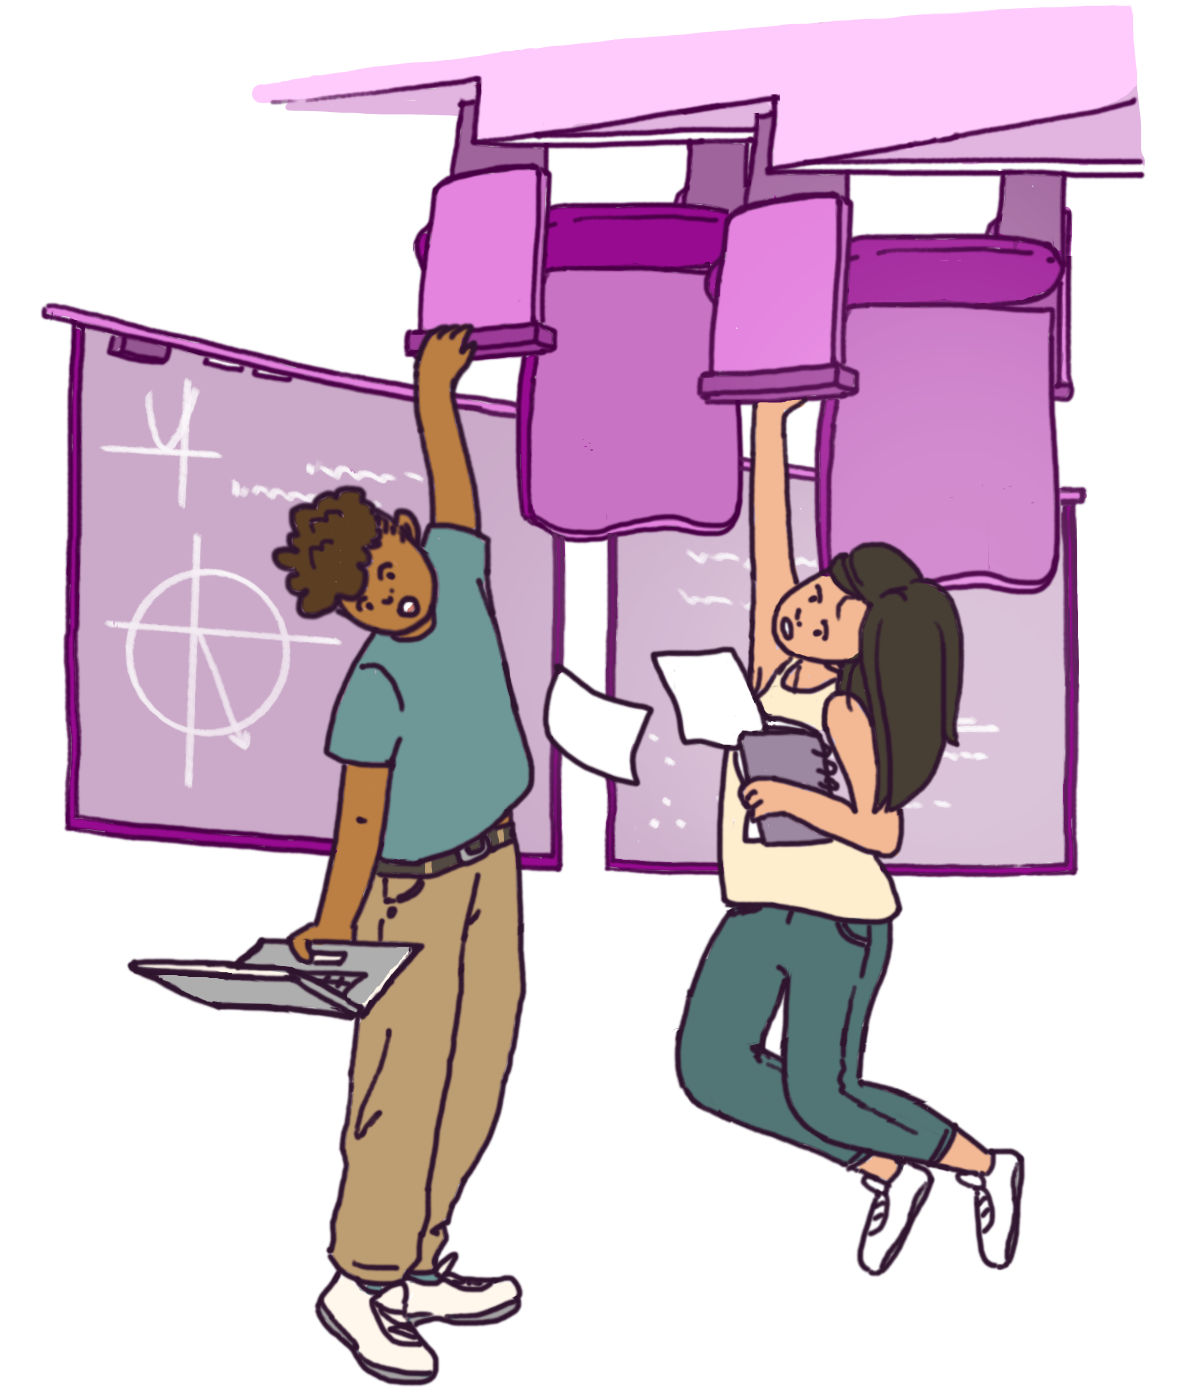
\includegraphics[width=1\linewidth]{Figuras/Fig01.png}
        \end{center}
    \end{columns}

\end{frame}

%%%%%%%%%%%%%%%%%%%%%%%%%%%%%%%%%%%%%%%%%%%%%%%%%%%%%%%%
\begin{frame}
    \begin{block}{Objetivo de la charla}
        \begin{itemize}[leftmargin=*]
            \item Presentar la metodología para integrar ChatGPT en el aula invertida.
            \item Motivar a replicar esta experiencia en otras asignaturas o contextos.
        \end{itemize}
    \end{block}

    \vspace{0.3cm}
    \pause
    \begin{block}{}\centering
        Caso de uso: Álgebra Lineal
    \end{block}
\end{frame}


%%%%%%%%%%%%%%%%%%%%%%%%%%%%%%%%%%%%%%%%%%%%%%%%%%%%%%%%
\fondo{celeste}
\section{¿Qué es la Metodología de Aula Invertida?}
\fondo{blanco}
%%%%%%%%%%%%%%%%%%%%%%%%%%%%%%%%%%%%%%%%%%%%%%%%%%%%%%%%


%%%%%%%%%%%%%%%%%%%%%%%%%%%%%%%%%%%%%%%%%%%%%%%%%%%%%%%%
\begin{frame}
    \frametitle{¿Qué es la Metodología de Aula Invertida?}
    \vspace{3mm}
    \begin{columns}
    \column{.4\textwidth}
    \begin{itemize}[leftmargin=*]
        \item Los estudiantes acceden a los contenidos antes de la clase.
        \item El tiempo en clase se dedica a actividades prácticas y resolución de problemas.
    \end{itemize}
    \column{.6\textwidth}
        \postitimg[0.99\linewidth]{Figuras/Fig02.png}
    \end{columns}
\end{frame}
%%%%%%%%%%%%%%%%%%%%%%%%%%%%%%%%%%%%%%%%%%%%%%%%%%%%%%%%


%%%%%%%%%%%%%%%%%%%%%%%%%%%%%%%%%%%%%%%%%%%%%%%%%%%%%%%%
\begin{frame}
    \frametitle{Particularidades del Aula Invertida}
    \begin{columns}
    \column{.5\textwidth}
    \begin{block}{Preclase:}
        \begin{itemize}
            \item Adquisición de conceptos.
            \item Personalización del contenido.
            \item Resolución  de dudas.
            \item Micro-tarea.
        \end{itemize}
    \end{block}
    \column{.5\textwidth}
    \begin{block}{En Clase:}
        \begin{itemize}
            \item Visión conjunta.
            \item Retroalimentación.
            \item Actividad de aplicación.
            \item Micro-evaluación.
        \end{itemize}
    \end{block}
    \end{columns}
\end{frame}
%%%%%%%%%%%%%%%%%%%%%%%%%%%%%%%%%%%%%%%%%%%%%%%%%%%%%%%%

%%%%%%%%%%%%%%%%%%%%%%%%%%%%%%%%%%%%%%%%%%%%%%%%%%%%%%%%
\begin{frame}
    \frametitle{Beneficios del Aula Invertida}
    \vspace{-5mm}
    \begin{columns}
    \column{.5\textwidth}
        \begin{center}
        \postitimg[0.99\linewidth]{Figuras/Fig03.jpg}
        \end{center}
    \column{.5\textwidth}
        \begin{itemize}[leftmargin=*]
            \item Mayor participación activa de los estudiantes.
            \item Aprendizaje más profundo y significativo.
            \item Flexibilidad en el ritmo de aprendizaje.
            \item Fomento del pensamiento crítico y la colaboración.
        \end{itemize}
    \end{columns}
\end{frame}
%%%%%%%%%%%%%%%%%%%%%%%%%%%%%%%%%%%%%%%%%%%%%%%%%%%%%%%%

%%%%%%%%%%%%%%%%%%%%%%%%%%%%%%%%%%%%%%%%%%%%%%%%%%%%%%%%
\begin{frame}
    \frametitle{Desafíos del Aula Invertida}
    \begin{columns}
    \column{.5\textwidth}
        \begin{itemize}[leftmargin=*]
            \item Resistencia al cambio por parte de estudiantes y docentes.
            \item Requiere una mayor preparación previa.
            \item Necesidad de acceso a recursos tecnológicos.
            \item Implementar mecanismos de evaluación continua.
        \end{itemize}
    \column{.5\textwidth}
        \begin{center}
        \postitimg[0.99\linewidth]{Figuras/Fig04.jpg}
        \end{center}
    \end{columns}
\end{frame}
%%%%%%%%%%%%%%%%%%%%%%%%%%%%%%%%%%%%%%%%%%%%%%%%%%%%%%%%

%%%%%%%%%%%%%%%%%%%%%%%%%%%%%%%%%%%%%%%%%%%%%%%%%%%%%%%%
\fondo{celeste}
\section{¿Qué es ChatGPT?}
\fondo{blanco}
%%%%%%%%%%%%%%%%%%%%%%%%%%%%%%%%%%%%%%%%%%%%%%%%%%%%%%%%

%%%%%%%%%%%%%%%%%%%%%%%%%%%%%%%%%%%%%%%%%%%%%%%%%%%%%%%%
\begin{frame}
    \frametitle{¿Qué es ChatGPT?}
    \begin{columns}
    \column{.55\textwidth}
        \postitimg[0.99\linewidth]{Figuras/Fig05.jpg}
    \column{.45\textwidth}
    \begin{itemize}[leftmargin=*]
        \item Modelo de lenguaje desarrollado por OpenAI.
        \item Mantiene conversaciones, responde preguntas, y asiste en tareas diversas.
        \item Funciona mediante el procesamiento de grandes volúmenes de texto para \textbf{predecir y generar respuestas} basadas en el contexto.
    \end{itemize}
    \end{columns}
\end{frame}
%%%%%%%%%%%%%%%%%%%%%%%%%%%%%%%%%%%%%%%%%%%%%%%%%%%%%%%%


%%%%%%%%%%%%%%%%%%%%%%%%%%%%%%%%%%%%%%%%%%%%%%%%%%%%%%%%
\begin{frame}
    \frametitle{Aplicaciones de ChatGPT en Educación}
    \begin{columns}
    \column{.35\textwidth}
        \begin{itemize}[leftmargin=*]
            \item Asistencia en la revisión de trabajos.
            \item Creación de materiales didácticos \textbf{personalizados}.
            \item Apoyo en la \textbf{tutoría} y resolución de dudas \textbf{en tiempo real}.
        \end{itemize}
    \column{.65\textwidth}
    \vspace{3mm}
        \postitimg[0.99\linewidth]{Figuras/Fig06.png}
    \end{columns}
\end{frame}
%%%%%%%%%%%%%%%%%%%%%%%%%%%%%%%%%%%%%%%%%%%%%%%%%%%%%%%%

%%%%%%%%%%%%%%%%%%%%%%%%%%%%%%%%%%%%%%%%%%%%%%%%%%%%%%%%
\fondo{celeste}
\section{Caso de uso}
\fondo{blanco}
%%%%%%%%%%%%%%%%%%%%%%%%%%%%%%%%%%%%%%%%%%%%%%%%%%%%%%%%

%%%%%%%%%%%%%%%%%%%%%%%%%%%%%%%%%%%%%%%%%%%%%%%%%%%%%%%%
\begin{frame}
    \frametitle{Caso de uso}

    \begin{itemize}
        \item \textbf{Asignatura:} Álgebra Lineal
        \item \textbf{Carrera:} Ciencia de Datos
        \item \textbf{Nivel:} Segundo nivel
        \item \textbf{Resultado de aprendizaje:} Resuelve operaciones con matrices, incluyendo productos, cálculo de inversas; además del  cálculo de determinantes de matrices, valores y vectores propios y su significado en el contexto del Álgebra Lineal.
    \end{itemize}
\end{frame}
%%%%%%%%%%%%%%%%%%%%%%%%%%%%%%%%%%%%%%%%%%%%%%%%%%%%%%%%

%%%%%%%%%%%%%%%%%%%%%%%%%%%%%%%%%%%%%%%%%%%%%%%%%%%%%%%%
\begin{frame}
\centering
    \postitimg[0.6\linewidth]{Figuras/Fig07.png}
\end{frame}
%%%%%%%%%%%%%%%%%%%%%%%%%%%%%%%%%%%%%%%%%%%%%%%%%%%%%%%%

%%%%%%%%%%%%%%%%%%%%%%%%%%%%%%%%%%%%%%%%%%%%%%%%%%%%%%%%
\begin{frame}
    \frametitle{Adquisición de concepto}

    \small

    Para la adquisición del concepto, se solicitará al estudiante interactuar con ChatGPT y la visualización de video, siguiendo los siguientes pasos:

\begin{enumerate}[leftmargin=*,label=\arabic*.]
    \item Interactuar con ChatGPT mediante los siguientes \textit{prompts}, leyendo detenidamente el \textit{prompt} y su respuesta:
    \begin{enumerate}[label=\textit{Prompt \arabic*.},leftmargin=2.1cm]
        \item Vas a ser mi profesor de la asignatura de Álgebra Lineal, te iré dando indicaciones y me irás explicando de manera formal lo que te pida. Vas a tener mucho cuidado al escribir la parte matemática para que se visualice bien. Sé divertido. ¿Entendido?
        \item ¿Cómo se calcula un valor propio de una matriz? No me des un ejemplo numérico aún.
        \item Dame un ejemplo del cálculo de valores propios con una matriz de 2 por 2.
    \end{enumerate}
\end{enumerate}
\end{frame}
%%%%%%%%%%%%%%%%%%%%%%%%%%%%%%%%%%%%%%%%%%%%%%%%%%%%%%%%

%%%%%%%%%%%%%%%%%%%%%%%%%%%%%%%%%%%%%%%%%%%%%%%%%%%%%%%%
\begin{frame}
    \frametitle{Adquisición de concepto}
\small
\begin{enumerate}[leftmargin=*,label=\arabic*.,start=2]
    \item Visualiza el siguiente video: \href{https://youtu.be/HET8XcIX-n4?si=t4lUbTmWaPOTbtAM}{Obteniendo los valores propios de una matriz de 2$\times$2}.
    \item Continúa la interacción con ChatGPT mediante los siguientes \textit{prompts}, leyendo detenidamente el \textit{prompt} y su respuesta:
    \begin{enumerate}[label=\textit{Prompt \arabic*.},leftmargin=2.1cm,start=4]
        \item Dame un ejemplo del cálculo de valores propios con una matriz de 3 por 3, que el ejemplo sea en una matriz triangular. Realízalo paso a paso con el cálculo de determinante.
        \item Plantéame un ejercicio de cálculo de valores propios en matrices de 2 por 2.
    \end{enumerate}
    \item Visualiza el video: \href{https://youtu.be/Gx0PaWI9eYo?si=oTPRSIfeEopspelW}{Vectores propios y valores propios}.
\end{enumerate}
\end{frame}
%%%%%%%%%%%%%%%%%%%%%%%%%%%%%%%%%%%%%%%%%%%%%%%%%%%%%%%%

%%%%%%%%%%%%%%%%%%%%%%%%%%%%%%%%%%%%%%%%%%%%%%%%%%%%%%%%
\begin{frame}
    \frametitle{Adquisición de concepto}
\small
\begin{enumerate}[leftmargin=*, label=\arabic*., start=4]
    \item Continúa la interacción con ChatGPT con las preguntas sobre el video que acabas de ver.
     \item En caso de tener más dudas sobre el tema, interactúa con tus compañeros de clase para solventarlas.
    \item Realiza el cuestionario del aula virtual.
\end{enumerate}
\end{frame}
%%%%%%%%%%%%%%%%%%%%%%%%%%%%%%%%%%%%%%%%%%%%%%%%%%%%%%%%

%%%%%%%%%%%%%%%%%%%%%%%%%%%%%%%%%%%%%%%%%%%%%%%%%%%%%%%%
\begin{frame}
    \begin{itemize}
        \item \textbf{Personalización de la actividad:}
        \begin{itemize}
            \item Estudiantes continúan interactuando con ChatGPT hasta asimilar completamente el concepto.
        \end{itemize}
        \item \textbf{Solventación de dudas:}
        \begin{itemize}
            \item Uso de ChatGPT para resolver dudas específicas sobre el tema y trabajo colaborativo con compañeros.
        \end{itemize}
        \item \textbf{Micro-tarea:}
        \begin{itemize}
            \item Estudiantes deben copiar el enlace del chat con ChatGPT como evidencia.
            \item Completar el cuestionario en el aula virtual.
        \end{itemize}
    \end{itemize}
\end{frame}
%%%%%%%%%%%%%%%%%%%%%%%%%%%%%%%%%%%%%%%%%%%%%%%%%%%%%%%%

%%%%%%%%%%%%%%%%%%%%%%%%%%%%%%%%%%%%%%%%%%%%%%%%%%%%%%%%
\begin{frame}
\centering
    \postitimg[0.75\linewidth]{Figuras/Fig08.png}\\
    {\footnotesize\url{https://chatgpt.com/share/59b3c97a-23da-4a56-8447-c23649c6f868}}
\end{frame}
%%%%%%%%%%%%%%%%%%%%%%%%%%%%%%%%%%%%%%%%%%%%%%%%%%%%%%%%

%%%%%%%%%%%%%%%%%%%%%%%%%%%%%%%%%%%%%%%%%%%%%%%%%%%%%%%%
\begin{frame}
\centering
    \postitimg[0.7\linewidth]{Figuras/Fig09.png}
\end{frame}
%%%%%%%%%%%%%%%%%%%%%%%%%%%%%%%%%%%%%%%%%%%%%%%%%%%%%%%%

%%%%%%%%%%%%%%%%%%%%%%%%%%%%%%%%%%%%%%%%%%%%%%%%%%%%%%%%
\begin{frame}
    \frametitle{Cuestionario en aula virtual}
    \begin{itemize}
        \item Copia el enlace del chat con ChatGPT como evidencia de la actividad realizada en casa.
        \item ¿Alguna pregunta que ChatGPT no te supo responder?
        \item En caso de que algún compañero te haya ayudado a resolver tus dudas, indica aquí quién o quienes te ayudaron.
        \item ¿Qué dudas tienes sobre calcular los valores propios de una matriz?
    \end{itemize}
\end{frame}
%%%%%%%%%%%%%%%%%%%%%%%%%%%%%%%%%%%%%%%%%%%%%%%%%%%%%%%%

%%%%%%%%%%%%%%%%%%%%%%%%%%%%%%%%%%%%%%%%%%%%%%%%%%%%%%%%
\begin{frame}
    \frametitle{Tareas en Clase y Evaluación}
    \begin{itemize}[leftmargin=*]
        \item \textbf{Visión conjunta:}
        \begin{itemize}
            \item Conectar actividades en casa con tareas en clase, enfocadas en el cálculo de vectores propios.
        \end{itemize}
        \item \textbf{Retroalimentación:}
        \begin{itemize}
            \item Feedback sobre las respuestas de la micro-tarea.
        \end{itemize}
        \item \textbf{Actividad de aplicación:}
        \begin{itemize}
            \item Ejercicios de cálculo de valores propios con matrices de diferentes tamaños.
        \end{itemize}
        \item \textbf{Micro-evaluación:}
        \begin{itemize}
            \item No se realiza una micro-evaluación específica en esta actividad.
        \end{itemize}
    \end{itemize}
\end{frame}
%%%%%%%%%%%%%%%%%%%%%%%%%%%%%%%%%%%%%%%%%%%%%%%%%%%%%%%%

\include{Secciones/05conclusiones}


%%%%%%%%%%%%%%%%%%%%%%%%%%%%%%%%%%%%%%%%
%% Página final
\fondo{final}
\begin{frame}[plain]
\begin{center}
    \color{white}
    
    \vspace{1.5cm}
    {\Huge\textbf{Gracias}}
    \vspace{2mm}
    

    \begin{tabular}{ccc}
        \href{https://linktr.ee/aemerinot}{
\includegraphics[width=2.5cm]{Figuras/QR-links.png}}
        &\phantom{.\hspace{.5cm}.}&
        \href{https://github.com/andres-merino/Presentacion-ChatGPT-AulaInvertida}{
\includegraphics[width=2.5cm]{Figuras/QR-presentacion.png}}
        \\
        \LARGE \faGithub\hspace{5mm} \faLinkedin%\hspace{5mm} \aiOrcidSquare 
        && 
        Presentación
    \end{tabular}

    \vspace{2mm}
    \textbf{Contacto:} aemerinot@puce.edu.ec
\end{center}
\end{frame}


\end{document}